\documentclass[a4paper,11pt]{report}

\usepackage{fullpage}
\usepackage{amsmath}
\usepackage{bussproofs}
\usepackage{color}
\usepackage{hyperref}
\usepackage{placeins}
\usepackage{csquotes}

\usepackage{etoolbox}
\usepackage[T1]{fontenc}
\usepackage[english]{babel}
\usepackage{array}
\usepackage{graphicx}
\usepackage{caption}
\captionsetup{font=footnotesize}

\usepackage[
    backend=biber,
    style=alphabetic,
    sortlocale=en_GB,
    natbib=true,
    url=false,
    doi=true,
    eprint=false,
    citestyle=alphabetic-verb
]{biblatex}


% % Page style
% \usepackage{fancyhdr}

% \setlength{\headheight}{17pt}
% \pagestyle{fancy}

% % Standard pages (inside chapters)
% \fancyhf{}
% \renewcommand{\headrulewidth}{0.4pt}
% \renewcommand{\footrulewidth}{0pt}
% \fancyheadoffset{0cm}

% \fancyhead[OR]{\bfseries \nouppercase{\rightmark}}
% \fancyhead[EL]{\bfseries \nouppercase{\leftmark}}
% \fancyfoot[EL,OR]{\thepage}

%%%%%%%%%%%%%%%%%%%%%%%%%%%%%%%%%%%%%%%%%%%%%%%%%%%%%%%%%
% Minted
%%%%%%%%%%%%%%%%%%%%%%%%%%%%%%%%%%%%%%%%%%%%%%%%%%%%%%%%%

\usepackage[cache=false]{minted}
\usemintedstyle{tango}

%%%%%%%%%% C
\newmintinline{c}{
    fontsize=\small,
    breaklines=true
}

\newminted{c}{
    frame=single,
    framesep=2mm,
    fontsize=\scriptsize,
    mathescape
}

\newminted[ccodeline]{c}{
    frame=single,
    framesep=2mm,
    fontsize=\scriptsize,
    mathescape,
    linenos
}


%%%%%%%%% CMAKE
\newminted{cmake}{
    frame=single,
    framesep=2mm,
    fontsize=\scriptsize,
    mathescape,
    linenos,
    breaklines=true
}

% End minted
%%%%%%%%%%%%%%%%%%%%%%%%%%%%%%%%%%%%%%%%%%%%%%%%%%%%%%%%%

\setlength{\parindent}{0pt}

\bibliography{bibliography}
\bibliographystyle{ieeetr}

\begin{document}
    \begin{center}
        \Large{
            Operating Systems\\
            Spring 2018
        }

        \noindent\makebox[\linewidth]{\rule{\linewidth}{0.4pt}}
        Operating Systems Project
        \noindent\makebox[\linewidth]{\rule{\linewidth}{0.4pt}}

        \begin{flushleft}
            Professor : Philippe Cudre-Mauroux

            Assistant : Ines Arous
        \end{flushleft}

        \noindent\makebox[\linewidth]{\rule{\linewidth}{0.4pt}}

        Submitted by Groupe 4: Sylvain Julmy, Michael Papinutto, Sami Veillard

        \noindent\makebox[\linewidth]{\rule{\textwidth}{1pt}}
        \vspace*{0.8cm}
        \today

    \end{center}

    \newpage

    \section*{Introduction}
    For this project, we implemented a multi-threaded client-server system using TCP sockets.

    One of the problem in designing such system is related to the database structure.
    Indeed, we can increase memory required but not time as this would impact User Experience.
    Hence, we tended to choose faster algorithm.
    Indeed, looking at applications usage revealed that sets are used in the following way: 90\% of calls are contains(),
    9\% are add() and 1\% are remove(). In this project, we selected a hash set for those reasons.
    Even though this system might require more memory resources and was rather complicated to implement, it was found to
    be efficient and powerful according to our test. Finally, our system has ability to write keys with values, read values
    providing a key, simultaneous safe access of the readers and the writers. This system was subsequently tested using
    an automated test in form of a bash script and text files of commands. This report mainly focus in explaining our
    approach as it was not part of the course and might be a strength of our project.


    \section*{Chosen approach}

    We had to keep in mind various aspect when choosing the data structure to
    store the key-value entry : maximal number of entry stored in the database,
    extension of the data structure, number of simultaneous access on the server and
    how to synchronize the threads.

    A lock-free hash-set data structure offers solutions to all of those challenges without blocking threads using mutex
    nor semaphores. We have implements our own data structure in C based on the one created by Herlihy in~\cite{Herlihy2006}
    in Java. Indeed, by using this implementation there is no need to prioritize neither read nor write action.

    Such implementation to be non-blocking requires atomic operations. Atomic operations are unique or multiple operations
    that cannot be stopped before their ends. In C, atomic operations such as CompareAndSet can be done by "stealing" a
    bit from a pointer using bit-wise operators to extract the pointer and the mark from a single word~\cite{Herlihy2006}.
    More Specifically, we used a reversed split-ordering hash set. A bucket is linked to a stack and as the list grow
    supplemental buckets references are added so that no object is ever too far from the start of a bucket, \textit{i.e.},
    the bucket size is kept small. This implementation ensures that when an item is put in the stack, it will not be
    moved. To do so, items have to be put in the stack using a recursive-split order. Moreover, to avoid
    problems occurring when deleting a node referenced by a bucket, a sentinel node is added at the beginning of each
    bucket. This special type of buckets are never deleted and can be identified by the Most Sensibel Bit which is set
    to 0 whereas for usual bucket is set to 1(see Figure~\ref{fig:Fig1}).

    \begin{figure}[h]
        \centering
            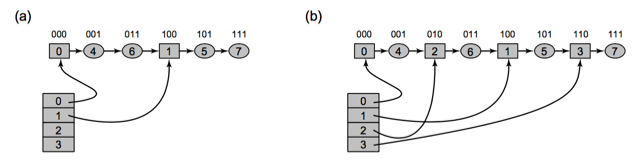
\includegraphics{images/hashsetFig1.png}
        \caption{Scheme of the recursive nature of the split ordering.
        The split order can be seen in binary words above buckets.
        Sentinel buckets are represented by square whereas ovals are normal buckets.
        (a) Shows a split-ordering including two buckets. The buckets are linked to a stack.
        (b) Shows how buckets are split in two part after the capacity of the table grows from 2 to 4.}
        \label{fig:Fig1}
    \end{figure}

    When inserting a new key in this data structure, the table is grown incrementally.
    As buckets are in a linked list ordered using split-ordering, the table resizing mechanism is independent to
    the threshold that decides when to resize. As the sets grows, most of the array will be use. Hence, when adding
    new values to a not yet initialized bucket that should have beeen initialized according to the current table capacity,
    this bucket will be initialized without generating an error. (see Figure~\ref{fig:Fig2}).


    \begin{figure}[h]
        \centering
            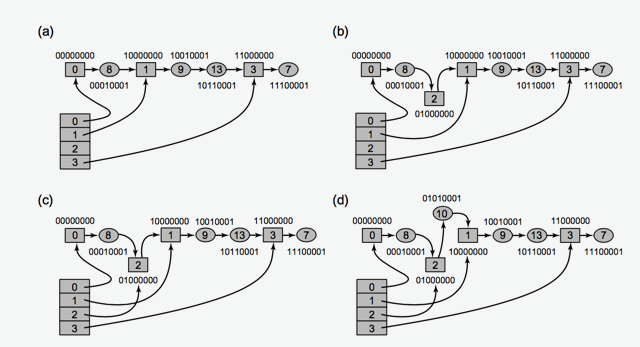
\includegraphics{images/hashsetFig2.png}
        \caption{Scheme of the procedure that add the key 10 to the lock-free hash set.
        As above, split-order key values are expressed in binary above buckets (here 8 bits words).
        (a) Buckets 0, 1 and 3 but bucket 2 is not.
        (b) An object with hash value of 10 is inserted to the set. This cause bucket 2 to be initialized and a new sentinel is inserted with split-order key 2.
        (c) Bucket 2 is affiliated with a new sentinel.
        (d) Finally, the split-order ordinary key 10 is added to bucket 2.}
        \label{fig:Fig2}
    \end{figure}

    In summary, our chosen approach implements a split-ordered hash set which is an array of buckets where each bucket
    is a reference to a lock-free list where nodes are sorted by their bit-reversed hash codes.
    The number of buckets grows dynamically, and each new bucket is initialized when accessed for the first time.

    \section*{Challenges encountered}
    One of the challenge we encountered was to read or deleted entries from values.
    Indeed, looking for a value in a hash-table is not as straight forward as it seems.
    It requires navigating through all the keys until the corresponding value is found.
    Despite the high cost of this operation, we decided to use this method as we did not find any other way to provide
    such an operation.

    Another challenge that we encountered was that we noticed using the implementation described above was not
    thread friendly.
    This problem was in fact due to the string tokenizer for commands was kept within an internal static variable. This
    issue was subsequently solved by reprogramming the tokenizer and further tested to ensure that thread kept their own
    tokenized command. This issue took us a lot of time and debugging to be solved.

    Finally, as only one of us was familiar with non-blocking operation and well versed in the intricacies of C programming,
    the other two had to keep up and learn a new way to program and think as this material was not presented
    during the class.

    \section*{Tests Results}
    We set up 3 test scenarii to evaluate our project: Collisions, No-Collisions ans Many Clients. In the Collisions scenario,
    we tested  11 clients and 28 commands (308 operations in total) using every operations available. In the No-Collisions
    scenario we tested 8 clients and 2700 commands (21600 operations in total). In the Many-Clients we tested 32 clients
    and 300 commands (9600 operations in total). In the No-Collisions and the Many-Clients scenarii we only used add, read
    value from key and delete key from value.

    \begin{centering}

        \begin{tabular}{|m{5cm}||m{3cm}|m{3cm}|m{3cm}|}\hline
            \multicolumn{4}{|c|}{Collision scenario}\\\hline\hline
           & Add & Read & Delete\\\hline
           Number of errors & 0 & 22 & 0 \\\hline
           Percentage of errors & 0\% & 7.14\% & 0\%\\\hline
        \end{tabular}

        \vspace{1cm}
        \begin{tabular}{|m{5cm}||m{3cm}|m{3cm}|m{3cm}|}\hline
            \multicolumn{4}{|c|}{No-Collision scenario}\\\hline\hline
           & Add & Read & Delete\\\hline
           Number of errors & 0 & 0 & 0 \\\hline
           Percentage of errors & 0\% & 0\% & 0\%\\\hline
        \end{tabular}

        \vspace{1cm}
        \begin{tabular}{|m{5cm}||m{3cm}|m{3cm}|m{3cm}|}\hline
            \multicolumn{4}{|c|}{Many-Clients scenario}\\\hline\hline
           & Add & Read & Delete\\\hline
           Number of errors & 0 & 0 & 0 \\\hline
           Percentage of errors & 0\% & 0\% & 0\%\\\hline
        \end{tabular}
    \end{centering}

    \vspace{1cm}
    Interestingly, the Many-Clients scenario required more time than the previous one despite it has half less operations.
    This is probably due to the synchronisation of clients requests.


    \section*{Conclusion}
    In conclusion, we addressed the challenges proposed in this project using a reversed split-ordering block-free
    hash-set data structure which offered us a way to cope with the prioritization of read and write operation.
    Moreover, as the usual operations use in a set was found to be mainly compose of contains and add, this
    implementation offered a fair trade off between between response time and memory pressure. However, such
    implementation does not prevent collisions but rather exhibits collision when entries were already deleted in the
    data structure also occuring in other implementations.


    \printbibliography

    \newpage

    \section*{Documentation}

    \subsection*{Communication}
    The server and the clients communicate through socket.

    \subsection*{Server}
    The server is composed of several binary files.
    The main file encompasses the socket setup for the server and dedicated files for communication and the shell
    graphical user interface.
    The server is multi-threaded, \textit{i.e.}, after each connection of a client the server create a new thread.
    The data structure is described above.


    \subsection*{Server usage}

    \begin{centering}
        \begin{tabular}{|m{3cm}|m{7cm}|}
            \hline
            TCP Port & 5000 (can be reset in the server main file) \\
            \hline
            .\textbackslash server & server start \\
            \hline
        \end{tabular}
    \end{centering}

    \subsection*{Client}
    The client is also composed of several binary files.
    The main file sets up client socket and dedicated files are used for execution of command and shell graphical
    interface.
    On the contrary of the server shell, the client shell is an interactive shell the usage thereof is described below.
    Moreover, to simplify benchmarking, the client can also accept files at launch.

    \subsection*{Client usage}

    \begin{centering}
        \subsubsection*{Client basic usage}
        \begin{tabular}{|m{6cm}|m{6cm}|}

            \hline
            .\textbackslash client <server ip address> & client start \\
            \hline
            .\textbackslash client -option <server ip address> & client start with options (see below) \\
            \hline
        \end{tabular}
        \subsubsection*{Options at start}
        \begin{tabular}{|m{4.5cm}|m{10.5cm}|}
            \hline
            \shortstack{-? \\ -h \\ -{}-help} & client command help \\
            \hline
            \shortstack{-f <file> \\ -{}-file <file>} & client start and execute command present in the file specified after this option \\
            \hline
            \shortstack{-F <file1> \ldots <fileN> \\ -{}-files <file1> \ldots <fileN>} & client start and execute command present in the files specified after this option \\
            \hline
        \end{tabular}

        \subsubsection*{Client command accepted in interactive GUI}
        \begin{tabular}{|m{7cm}|m{8cm}|}
            \hline
            add <value> or add <key> <value> & adds a value to the database with or without a generated key \\
            \hline
            ls & lists the content of the database (unordered) \\
            \hline
            read\_v <key> & reads a value in the database from a key \\
            \hline
            read\_k <value> & reads a key in the database from a value \\
            \hline
            rm\_v <key> & deletes a value in the database from a key \\
            \hline
            rm\_k <value> & deletes a value in the database from a key \\
            \hline
            update\_kv <value> <newvalue> & updates an entry in the database \\
            \hline
        \end{tabular}
    \end{centering}

\end{document}